\documentclass[twocolumn,10pt]{article}

\usepackage[a4paper,hmargin=1.5cm,vmargin=2.5cm,]{geometry}
\setlength{\columnsep}{0.7cm}
\usepackage{palatino}
\usepackage{graphicx}
\usepackage[utf8]{inputenc}
\usepackage{hyperref}
\urlstyle{same} % no tt font for URLs

\usepackage{natbib}
\bibliographystyle{genome_research}
%\setcitestyle{aysep={}} 

\usepackage[dvipsnames]{xcolor}
\hypersetup{
    colorlinks,
    linkcolor={blue!50!black},
    citecolor={blue!50!black},
    urlcolor={blue!50!black}
}
\renewcommand{\dbltopfraction}{0.7}
\renewcommand{\textfraction}{0.2}

\begin{document}

\setcounter{secnumdepth}{0}

\twocolumn[{%
\centering
\textbf{\Large Analysing single-cell bisulfite sequencing data with scbs}
\vspace{1.5ex}

Lukas P. M. Kremer, Leonie Küchenhoff, ..., Simon Anders\\
{\footnotesize University of Heidelberg, Germany}
\vspace{1.5ex}

November 2021
\vspace{6ex}
}]

\section{Abstract}

[...]

\section{Introduction}

Sequencing-based assays with single-cell resolution have offered new means to understand the differences between the cells making up a sample. Single-cell RNA sequencing techniques have matured at great pace in recent years, and methods to study chromatin are rapidly catching up. Of special interest here is DNA methylation, i.e., the methylation of bases in the DNA, because DNA methylation patterns are passed on to daughter cells in cell division. Especially in mammals, such methylation chiefly occurs at cytosine bases that are immediately after followed by guanine bases, so-called CpG sites. 

To detect CpG methylation by sequencing, bisulfite conversion is commonly employed: treatment of DNA with bisulfite causes unmethylated guanine bases to be deaminated to uracil, which is paired with thymine in subsequent PCR. Therefore, unmethylated CpGs are read as TG in sequencing of bisulfite-converted DNA while only methylated CpG is correctly read as CG \citep{Frommer_1992}. Such so-called bisulfite sequencing has been used for bulk samples since long, and methods for bisulfite sequencing with single-cell resolution \citep{Smallwood_2014} have become commercially available recently and are increasingly used.

CpG dinocleotides are underrepresented in eukariotic genomes (due to their vulnerability to mutation by conversion to TpG due to accidental deanimation), and the majority of existing CpG sites are methylated. Presence or absence of the methyl group at CpG sites is believed to have effect on gene regulation, with methylation inhibiting transcription. Methylating DNA during differentiation is therefore conjectured to be an important mechanism to silence genome regions that are not needed in the target lineage. One important application of single-cell bisulfite sequencing (sc-BS-Seq) therefore lies in the study of differentiation processes.

In the present paper, we discuss strategies to analyse sc-BS-Seq data, suggest improvement to current approaches, show their value in a benchmark, and present software to perform the improved analysis methods.

\section{Standard approach}

We start by briefly reviewing the standard approach of analysing single-cell \emph{RNA}-Seq data, and how this approach is typically adapted to the case of DNA methylation data.

The starting point in scRNA-Seq is a matrix of UMI counts (i.e. of counts of distinct RNA molecules), one row for each cell and one column for each gene. As a first step towards assigning cell types or states to cells, one needs to establish which cells are similar to each other, and to this end, find a way to quantify the distance (i.e., dissimilarity) between any two given cells' transcriptional profile. A standard approach, used with minor variation in virtually all recent research and automated by popular software such as Seurat or ScanPy, is as follows: One first accounts for cell-to-cell variation in sequencing depth by dividing each UMI count by the respective cell's total UMI count, then transforms to a homoskedastic scale by taking the logarithm. In order to avoid matrix elements with zero count to be transformed to minus infinity, one typically adds a very small ``pseudocount'' (often $10^{-5}$) to the normalized fractions before taking the logarithm. Now, one could use Euclidean distances of these vectors  of logarithmized fractions as dissimilarity score. However, these scores would be exceedingly noisy due to the strong Poisson noise introduced by the many genes with very low counts. Therefore, one performs a principal component analysis (PCA), keeping only the top few (typically, 20 to 50) components. As Poisson noise is uncorrelated between genes, it will average out in the top principal components. Therefore, Euclidean distances between these "PCA space" vectors provide a robust dissimilarity score, which can subsequently be used as input to methods like t-SNE and UMAP, which provide a two-dimensional representation of the data. The PCA space representation is furthermore used for clustering (assigning cells to groups by similarity) and trajectory finding (identifying elongated manifolds in PCA space and assigning cells to quasi-1D positions along them).

This procedure is commonly adapted when working with single-cell DNA-methylation data, so that all the tools used in scRNA-Seq downstream of the PCA step can be used. The question is therefore how to construct a suitable matrix as input for the PCA. A simple and popular approach is to tile the genome into windows of, say, 100 kB size, and calculate for each cell the average methylation of the DNA within each window. To this end, we identify all CpG sites in the window for which we have coverage with at least one read and can hence call the CpG to be either unmethylated or methylated in the cell. Then we denote as average DNA methylation of this window in a given cell the proportion of observed CpG sites in the window have been found to be methylated. This yields a matrix, with one row for each cell and one column for each window from the genome tiling, comprising numbers (methylation fractions) between 0 and 1. This matrix is now subjected to PCA.

As an example, we will us in this paper data from XX et al., who have performed sc-BS on [...] and analysed their data in the manner just described. Figure 1a shows a UMAP plot, derived from our re-analysis of the data, using a tiling of the genome into windows of size 100 kb. As one can see, the approach is suitable to see clear structure in the data, observe ...

Nevertheless, this analysis strategy has substantial room for improvement, as we will discuss next.

\begin{figure}
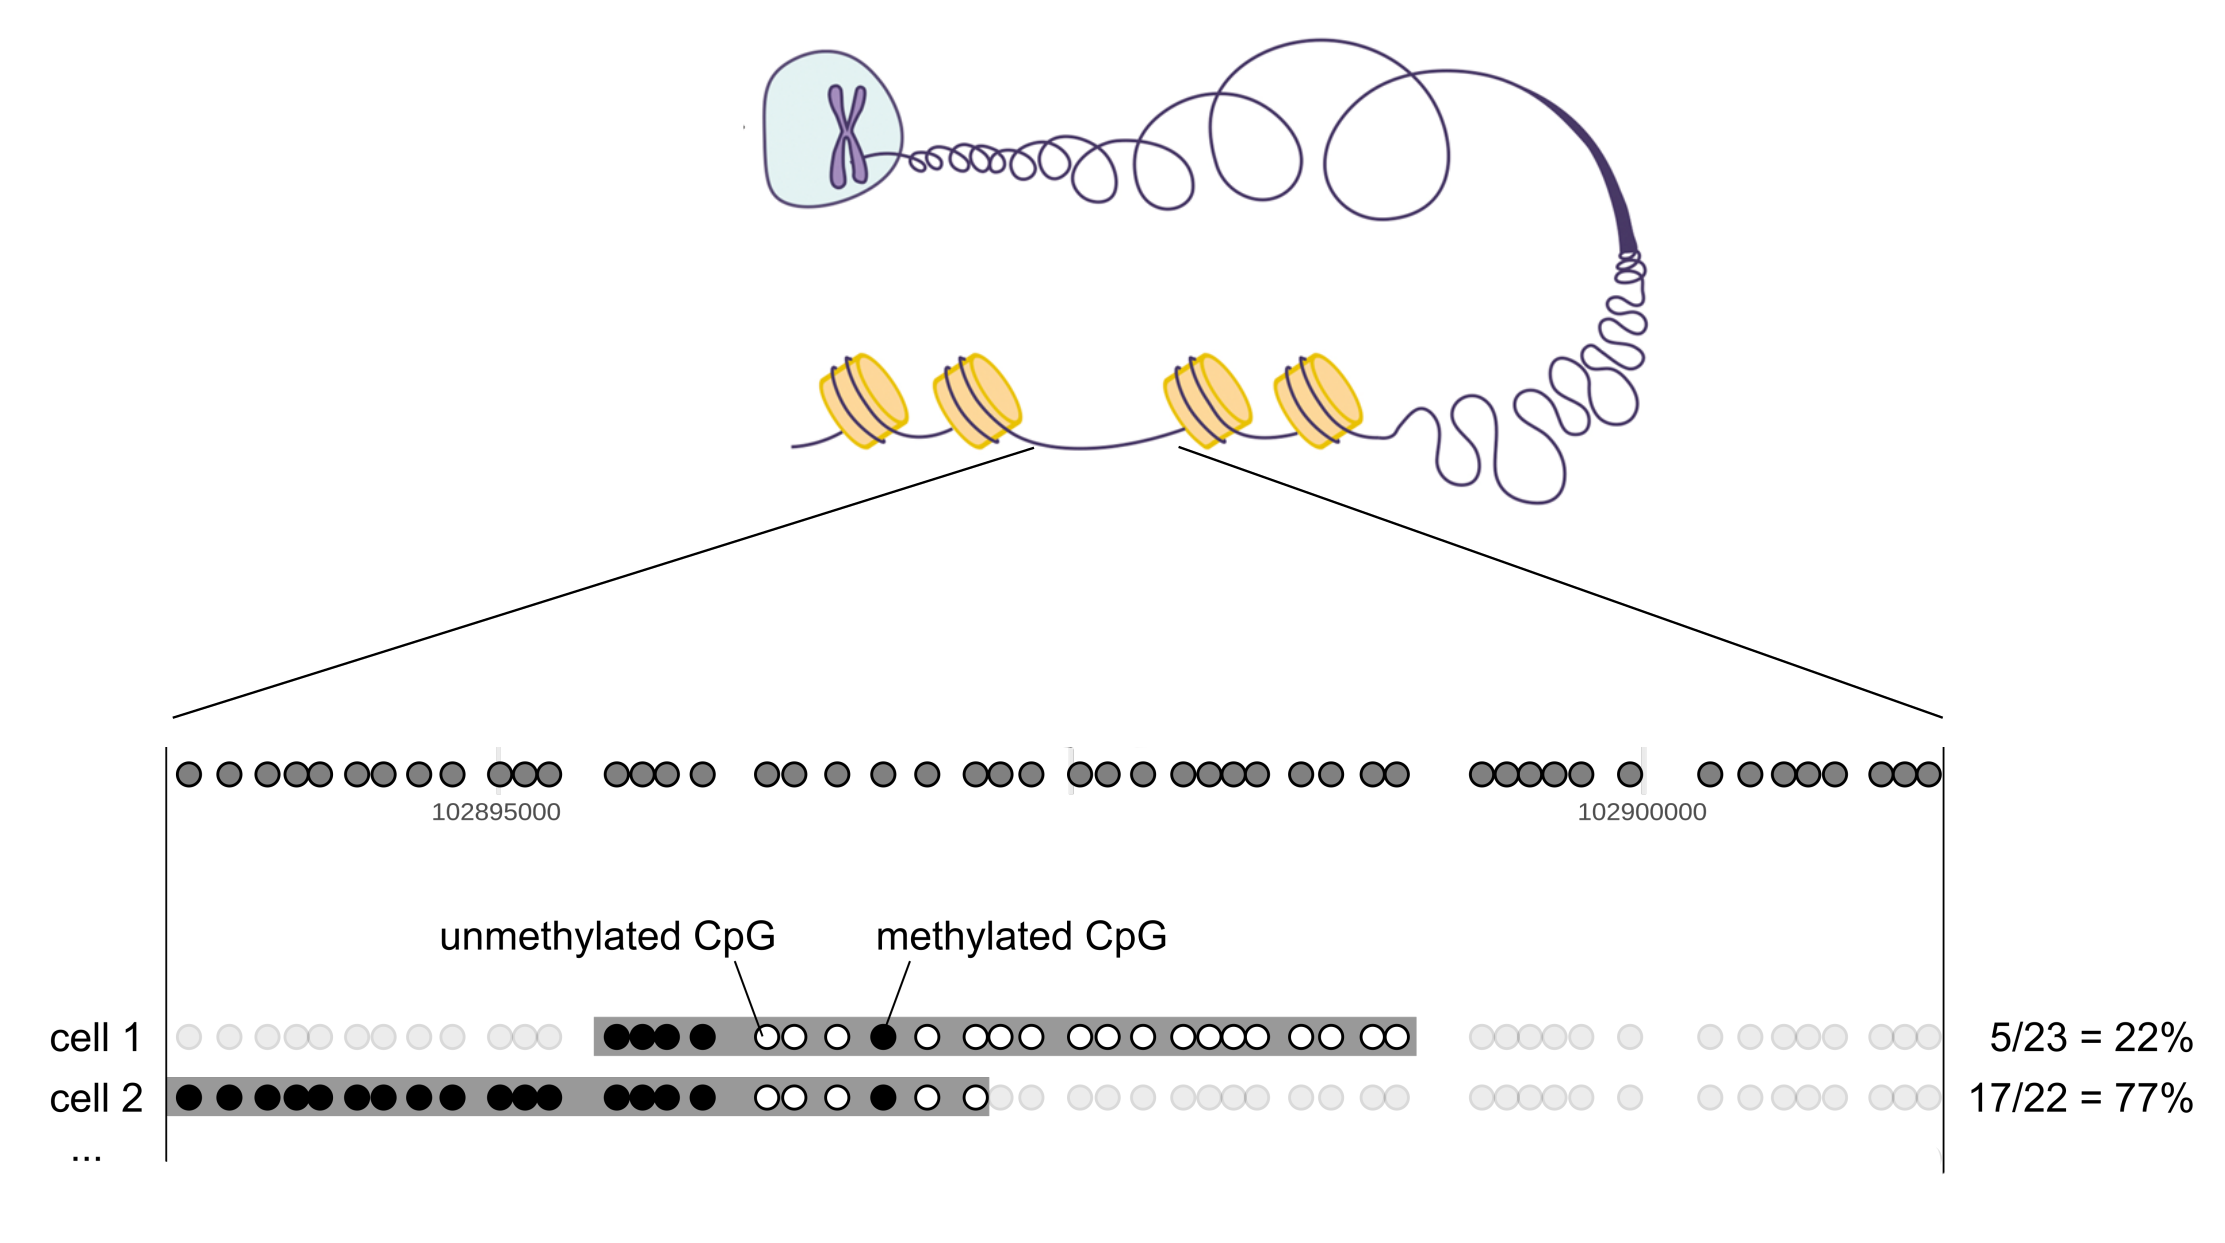
\includegraphics[width=\columnwidth]{need_for_relative_meth.png}
\caption{\textbf{Effect of read position:} Depicted is a genomic interval along a chromosome, for which DNA methylation is to be quantified. Two cells cover differing parts of the interval with one read each. If one simply counts for each cell which fraction of the covered CpG sites are methylated, one obtains very different values for the two cells.}
\end{figure}

\section{Read position affects average}


\end{document}